\subsection{The exponent really is \texorpdfstring{$\min(c(1-\gamma), 1/2)$}{min(c(1-gamma), 1/2)}}

We ran TD(0) on the robot (policy s/re, $\gamma = 0.8$) for $10^6$ updates with $\alpha_n = c/(n+c-1)$ and ten values of $c$, 30 seeds each. The error is $\max_s |V(s) - v(s)| / \max_s |v(s)|$ and we fit the slope of $\log(\text{mean error})$ against $\log n$ between $10^4$ and $10^6$ updates.

\begin{table}[htbp]
\centering\small
\setlength{\tabcolsep}{3.5pt}
\begin{tabular}{lcccccccccc}
\toprule
$c$ & 0.5 & 1 & 1.5 & 2 & 2.5 & 3 & 4 & 5 & 10 & 20 \\
\midrule
predicted slope & $-0.10$ & $-0.20$ & $-0.30$ & $-0.40$ & $-0.50$ & $-0.50$ & $-0.50$ & $-0.50$ & $-0.50$ & $-0.50$ \\
measured slope & $-0.100$ & $-0.200$ & $-0.301$ & $-0.402$ & $-0.506$ & $-0.604$ & $-0.518$ & $-0.504$ & $-0.555$ & $-0.483$ \\
$10^3 \times$ final error & 180 & 52 & 15.2 & 4.7 & 1.39 & 0.48 & 0.30 & 0.34 & 0.29 & 0.44 \\
\bottomrule
\end{tabular}
\caption{Slope of the error in log-log scale for $\alpha_n = c/(n+c-1)$, robot, $\gamma = 0.8$, 30 seeds.}
\label{tab:phase}
\end{table}

\begin{figure}[htbp]
\centering
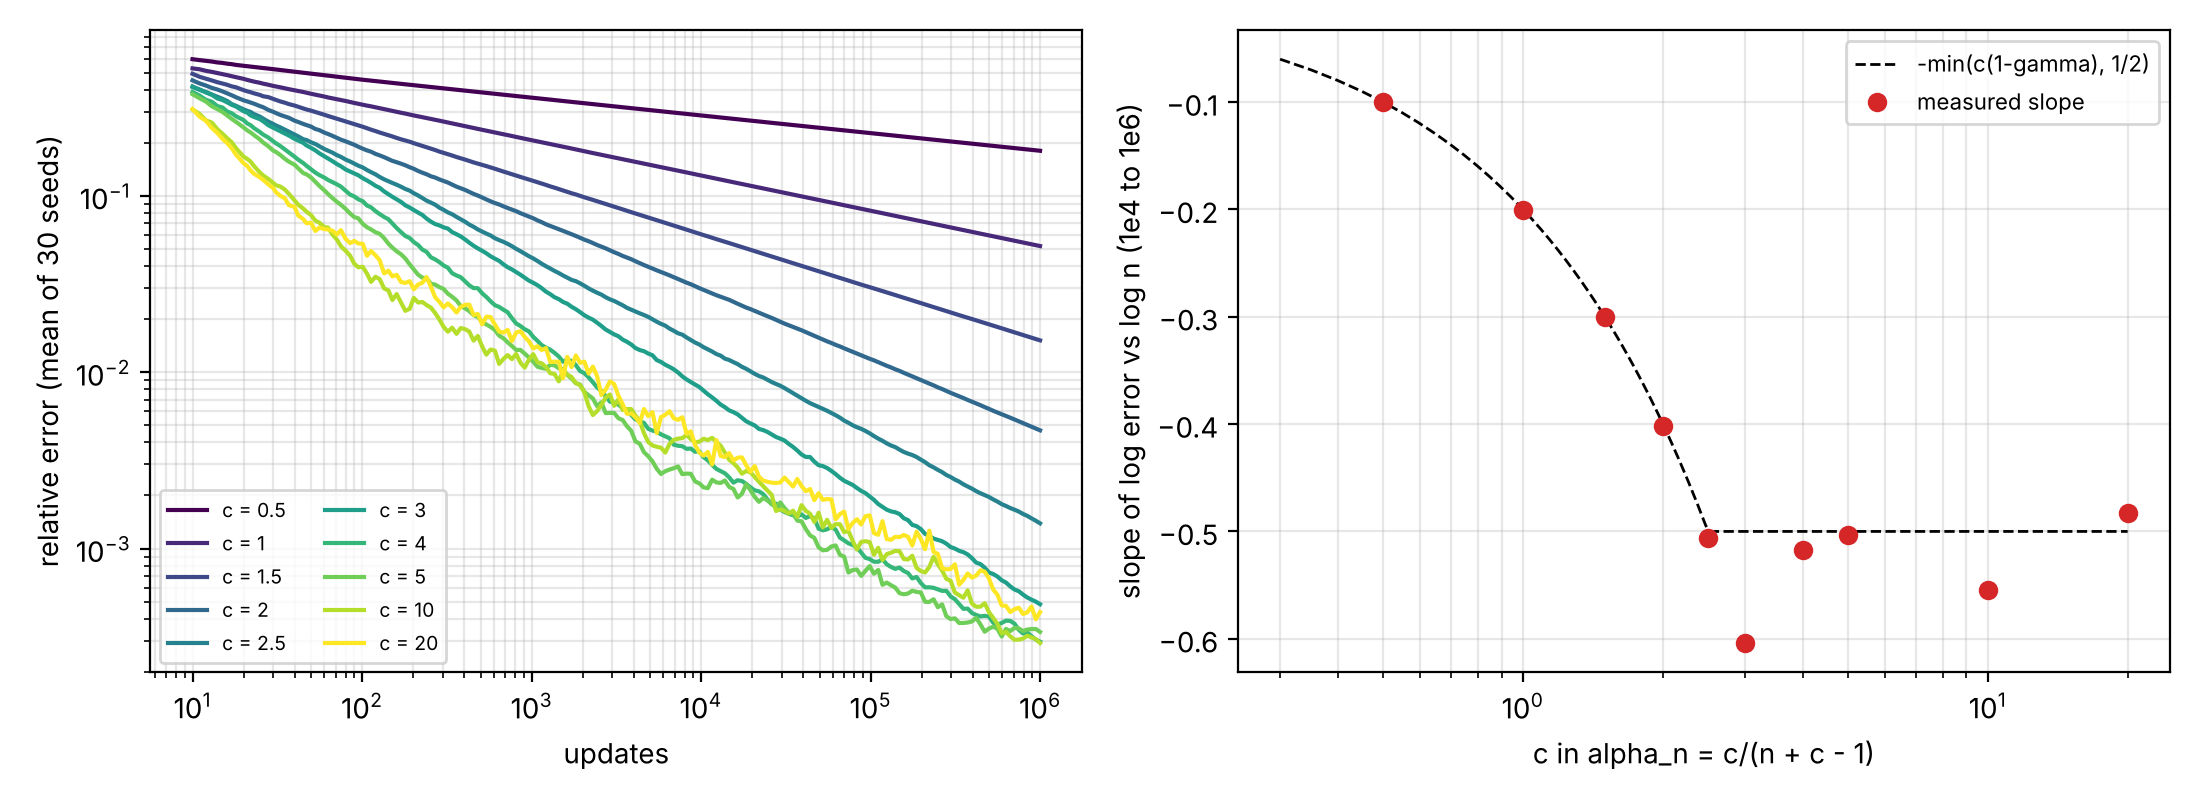
\includegraphics[width=\textwidth]{steps_phase.png}
\caption{Left: relative error of TD(0) for different $c$. Right: measured slope against the prediction $-\min(c(1-\gamma), 1/2)$.}
\label{fig:phase}
\end{figure}

We did not expect the agreement to be this good. Up to $c = 2.5$ the slopes match the prediction to the second decimal (Table~\ref{tab:phase} and Figure~\ref{fig:phase}). In this regime the error is almost deterministic, it is the bias of $V_0 = 0$ that decays, so in a way the one-state calculation is exactly what is measured. Above $c = 2.5$ we are in the noise regime and the slopes scatter around $-0.5$, between $-0.48$ and $-0.60$. The value $-0.60$ at $c = 3$ is because the bias term $n^{-0.6}$ is still larger than the noise in our window, it would go to $-0.5$ later.

So the step $1/n$ of the report is not ``slow'' in some vague sense. It sits at $c(1-\gamma) = 0.2$, deep in the regime where the initial error is forgotten at speed $n^{-0.2}$. Just taking $c = 4$ instead of $c = 1$ divides the final error by about 175. Very large $c$ is a bit worse again ($c = 20$ gives $4.4 \times 10^{-4}$), because the noise constant grows with $c$.

\subsection{How the cost grows with the horizon}

Next we changed $\gamma$ from $0.5$ to $0.98$, so the effective horizon $H = 1/(1-\gamma)$ goes from 2 to 50, and counted how many updates are needed before the mean relative error goes below $5\%$ and stays there. The budget is $10^6$ updates. Four rules are compared: $1/n$, $H/(n+H-1)$ (that is $c = H$), $1/n^{0.8}$ and $1/n^{0.6}$.

\begin{table}[htbp]
\centering\small
\begin{tabular}{lcccccc}
\toprule
$\gamma$ & 0.5 & 0.7 & 0.8 & 0.9 & 0.95 & 0.98 \\
$H$ & 2 & 3.3 & 5 & 10 & 20 & 50 \\
\midrule
$1/n$ & 135 & 6\,905 & -- & -- & -- & -- \\
\quad one-state prediction & 127 & $9.1\times 10^{3}$ & $1.5\times 10^{6}$ & $5\times 10^{12}$ & $6\times 10^{25}$ & $6\times 10^{64}$ \\
$H/(n+H-1)$ & 31 & 80 & 143 & 340 & 766 & 1\,825 \\
$1/n^{0.8}$ & 42 & 286 & 1\,366 & 27\,682 & 629\,498 & -- \\
$1/n^{0.6}$ & 37 & 85 & 191 & 1\,084 & 5\,805 & 58\,727 \\
\bottomrule
\end{tabular}
\caption{Number of updates before the relative error stays under $5\%$ (mean of 30 seeds). A dash means not reached within $10^6$ updates.}
\label{tab:horizon}
\end{table}

\begin{figure}[htbp]
\centering
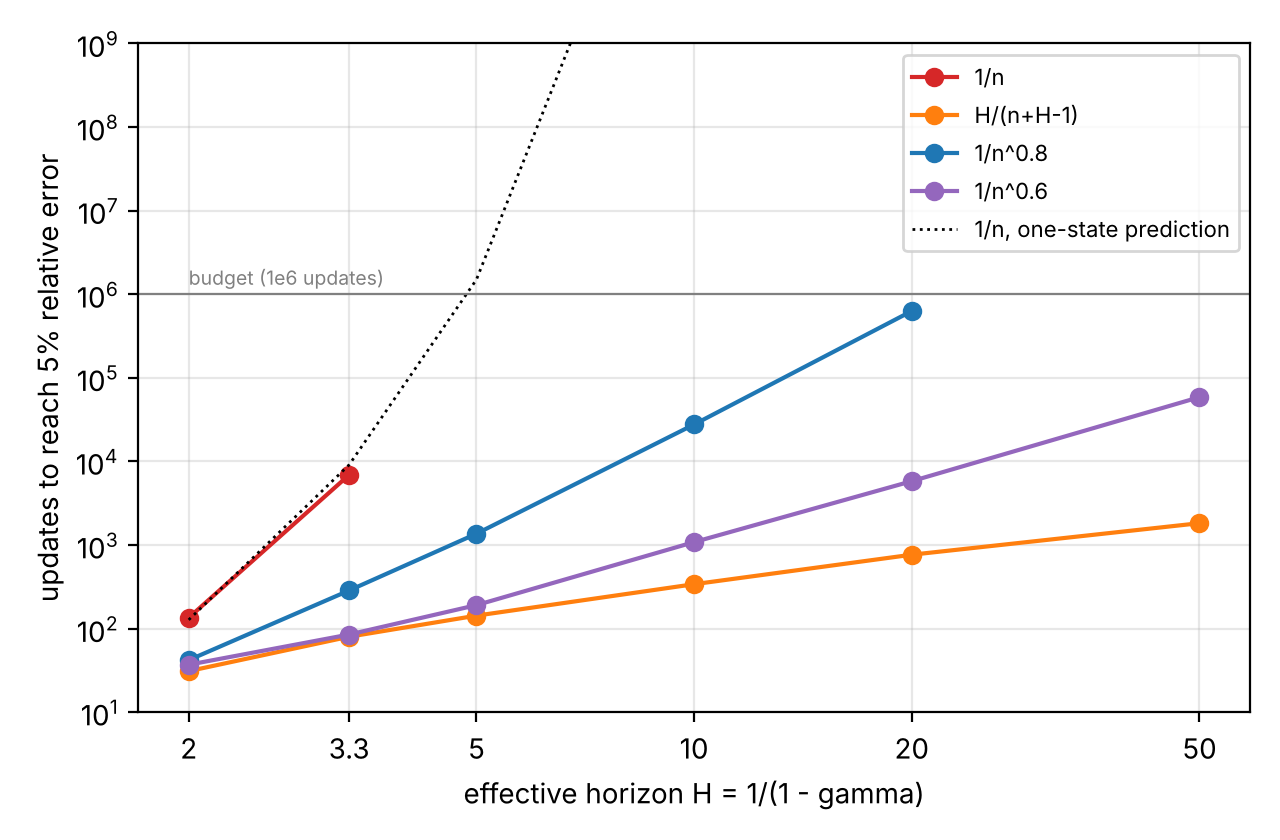
\includegraphics[width=0.72\textwidth]{steps_horizon.png}
\caption{Updates needed to reach $5\%$ relative error as a function of the horizon (log-log). The dotted line is the one-state prediction for $1/n$.}
\label{fig:horizon}
\end{figure}

Table~\ref{tab:horizon} is basically the Even-Dar and Mansour story on one small example. With $1/n$ the one-state formula $n \approx (0.05\,\Gamma(\gamma))^{-1/(1-\gamma)}$ predicts 127 updates for $\gamma = 0.5$ and about 9\,100 for $\gamma = 0.7$, we measure 135 and 6\,905. For $\gamma = 0.8$ it predicts $1.5 \times 10^6$, just above our budget, and indeed the error at $10^6$ is $5.2\%$, so it misses by very little. Beyond that the predicted numbers are astronomical, $5 \times 10^{12}$ updates for $\gamma = 0.9$, and of course nothing happens.

The rule $c = H$ is the opposite: the cost grows roughly linearly with the horizon, from 31 updates for $H = 2$ to 1\,825 for $H = 50$ (a fit in log-log gives a power of $1.25$). The polynomial steps are in between. They are polynomial in $H$ as promised, but the power can be large. For $1/n^{0.8}$ the bias calculation gives $n \approx ((1-\omega)\,H \log 20)^{1/(1-\omega)}$, so roughly $(0.6\,H)^5$. That is $7.7 \times 10^3$ for $H = 10$ and $2.5 \times 10^5$ for $H = 20$; we measure about three times more, which is the right order. With $\omega = 0.6$ the power is only $2.5$ and the rule reaches the target even for $H = 50$.

\subsection{Which \texorpdfstring{$\omega$}{omega}?}

If one does not want to depend on $\gamma$, a polynomial step $1/n^\omega$ is tempting. Figure~\ref{fig:omega} shows the relative error after $10^5$ updates (averaged over the second half of the run and over 30 seeds) for $\omega$ from $0.5$ to $1$ and the same six values of $\gamma$.

\begin{figure}[htbp]
\centering
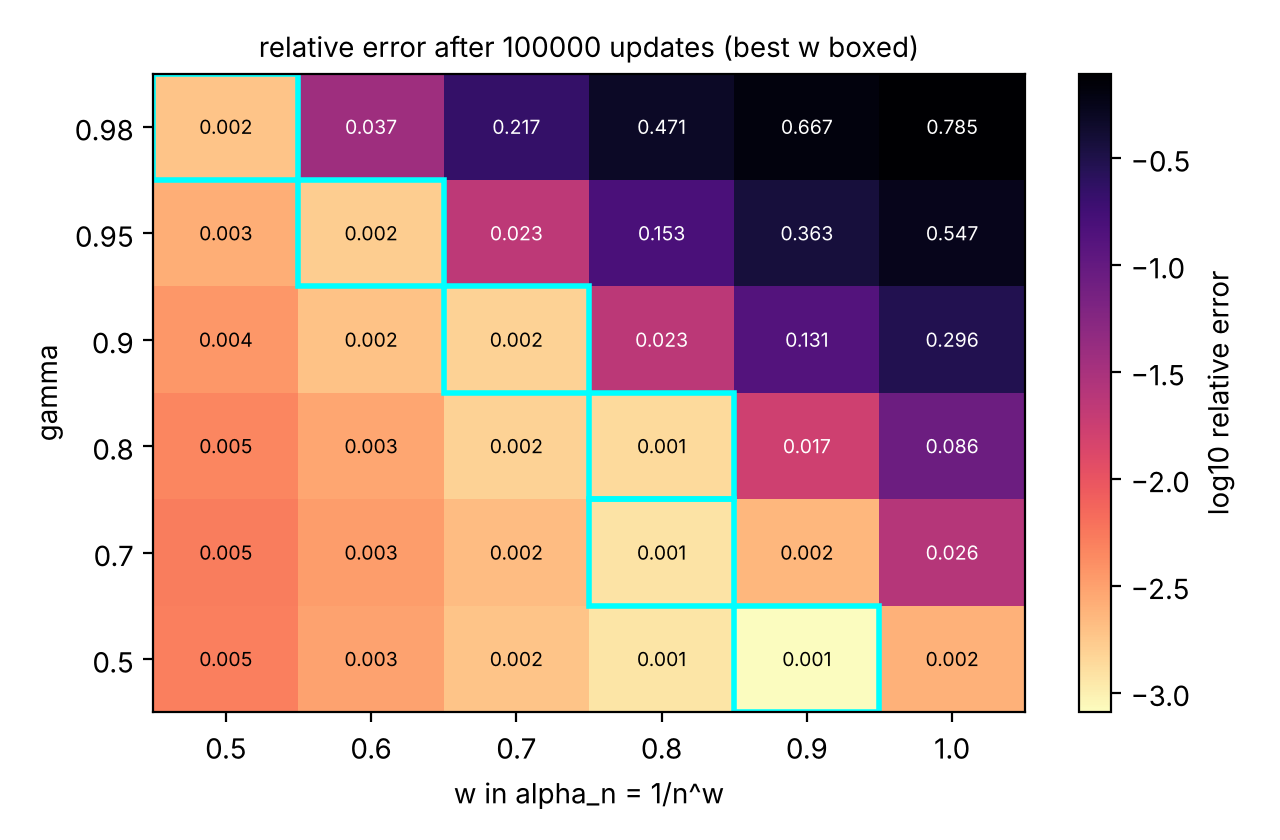
\includegraphics[width=0.66\textwidth]{steps_omega.png}
\caption{Relative error after $10^5$ updates with $\alpha_n = 1/n^\omega$. The best $\omega$ for each $\gamma$ is boxed.}
\label{fig:omega}
\end{figure}

The best $\omega$ goes down regularly when the horizon grows: $0.9$ for $\gamma = 0.5$, $0.8$ for $0.7$ and $0.8$, $0.7$ for $0.9$, $0.6$ for $0.95$ and $0.5$ for $0.98$. This is what the bias-variance argument says. A longer horizon means the bias is forgotten more slowly, so one needs larger steps (smaller $\omega$) and accepts a bit more noise. The cost of a wrong $\omega$ is very asymmetric. In our grid, taking $\omega$ too small costs at most a factor of about $6$, while taking it too large can cost more than two orders of magnitude ($0.785$ against $0.0019$ for $\gamma = 0.98$).

One funny detail: $\omega = 0.5$ has the best worst case of the whole grid (at most $0.0053$), but it is outside the Robbins--Monro conditions since $\sum_n 1/n$ diverges, so nothing guarantees it converges. For a fixed budget it does not matter much. If $\gamma$ is known, the rule $c/(n+c-1)$ with $c$ around $H$ is still the simplest choice, it reached $2$ to $3 \times 10^{-4}$ relative error after $10^6$ updates for every $\gamma$ we tried.
